
\documentclass{article}

% if you need to pass options to natbib, use, e.g.:     
\PassOptionsToPackage{numbers, compress}{natbib}

% to compile a preprint version, e.g., for submission to arXiv, add add the
% [preprint] option:
%     \usepackage[preprint]{neurips_2024}


% to compile a camera-ready version, add the [final] option, e.g.:



% to avoid loading the natbib package, add option nonatbib:
%    \usepackage[nonatbib]{neurips_2024}

\usepackage[final]{neurips_2024}
\usepackage[utf8]{inputenc} % allow utf-8 input
\usepackage[T1]{fontenc}    % use 8-bit T1 fonts
%\usepackage{hyperref}       % hyperlinks
\usepackage{url}            % simple URL typesetting
\usepackage{booktabs}       % professional-quality tables
\usepackage{amsfonts}       % blackboard math symbols
\usepackage{nicefrac}       % compact symbols for 1/2, etc.
\usepackage{microtype}      % microtypography
\usepackage{xcolor}         % colors
\usepackage{amsmath}
%\usepackage{neurips_2024}
\usepackage{graphicx}
\usepackage{wrapfig}
\usepackage{todonotes}
\usepackage{algorithm}
\usepackage{algpseudocode}
\usepackage{authblk}
\usepackage{caption}
\usepackage[hidelinks]{hyperref}
\usepackage{float}
\usepackage{wrapfig}

\title{RAG Question-Answer System}



% The \author macro works with any number of authors. There are two commands
% used to separate the names and addresses of multiple authors: \And and \AND.
%
% Using \And between authors leaves it to LaTeX to determine where to break the
% lines. Using \AND forces a line break at that point. So, if LaTeX puts 3 of 4
% authors names on the first line, and the last on the second line, try using
% \AND instead of \And before the third author name.


\setlength{\affilsep}{1em} % Adjust space between authors and affiliation


\author{%
  \begin{minipage}[t]{0.48\textwidth}
    \centering
    Lohith Sasanapuri \\
    \href{mailto:lsasanapuri@tulane.edu}{lsasanapuri}@tulane.edu
  \end{minipage}
  \hfill
  \begin{minipage}[t]{0.48\textwidth}
    \centering
    Pavan Kumar Sanjay \\
     \href{mailto:psanjay@tulane.edu}{psanjay}@tulane.edu
  \end{minipage}
}


\affil[]{
    \textbf{Department of Computer Science} \\
    Tulane University, New Orleans, LA \\   
}



\begin{document}
\maketitle
\section{Abstract}
Conventional chatbots often face challenges in maintaining a natural conversational flow and delivering precise, factual information. This study investigates chatbots based on retrieval-augmented generation (RAG), which have the potential to be more efficient and user-friendly. By considering the resource demands of large language models (LLMs) within the RAG framework, we have implemented a system based on the Retrieval-Augmented Generation for Knowledge-Intensive Natural Language Processing Tasks\cite{RAG_lewis}, which necessitates minimal retraining or fine-tuning of the LLMs utilized. Our objective was to create a chatbot that requires few training resources while ensuring high levels of accuracy. This report outlines our approach, findings, and the efficacy of our RAG-based chatbot.

\section{Introduction}
Conventional chatbot systems face challenges in delivering a natural conversational experience, particularly in comprehending user input. Operating primarily on static, rule-based frameworks limits their ability to enhance responses and often results in difficulties when providing fact-based answers. This rigidity can lead to a disjointed user experience. 

To address these shortcomings, advanced AI-based architectures, such as Retrieval-Augmented Generation (RAG), are emerging as advantageous solutions to develop more capable chatbots. This architecture leverages retrieval capabilities to extract relevant context from prior conversations or associated documents. In addition, it employs the generative qualities of large language models (LLMs) to facilitate more accurate, contextually relevant, and fact-based dialogues, with the aim of a more comprehensive understanding of user needs.

Although various RAG architectures have been proposed recently, this study focuses on a specific architecture from the \textit{RAG Lewis} \cite{RAG_lewis}, which is designed for tasks involving natural languages. This architecture requires minimal to zero retraining, yet it strives to deliver competitive performance.

We aim to implement this architecture to create a chatbot and evaluate its effectiveness in providing accurate and contextually relevant responses with minimal to no retraining, ultimately demonstrating its potential as a significant improvement over traditional chatbot systems.

\section{Related Work}
    Previous research has extensively explored how to equip large language models (LLMs) with up-to-date knowledge to address issues like factual accuracy and knowledge base limitations. The\textit{RAG Lewis} \cite{RAG_lewis} in "Retrieval-Augmented Generation for Knowledge-Intensive NLP Tasks," presented a significant advancement in this area. Their proposed RAG system distinguishes itself by requiring minimal to zero task-specific retraining or fine-tuning. It employs a dense retrieval component, trained using a pre-trained frequency model, to identify and extract relevant information from an external knowledge source. This retrieved information is then used to augment the input to a generative model, enabling the generation of fact-based conversational responses. The RAG architecture's ability to perform effectively on knowledge-intensive tasks without extensive retraining makes it a particularly relevant foundation for our work, where we aim to develop a chatbot that can provide accurate information with minimal adaptation.
    
   Building upon the principles of retrieval-augmented generation, the development of ChatDiet, as described by Yang et al. (2023) in "ChatDiet: Empowering personalized nutrition-oriented food recommender chatbots through an LLM-augmented framework"\cite{ChatDiet} demonstrates the application of a RAG-like architecture for personalized conversational agents. ChatDiet leverages retrieval technology to provide personalized nutrition-oriented food recommendations to users. The system operates by accessing two primary databases: a personal model database containing user-specific information and a population-based database with nutritional elements. Upon receiving a user query, ChatDiet retrieves relevant information from these databases and passes it as context to a large language model. The LLM then generates a response tailored to the user's nutritional needs and preferences based on the retrieved information. This approach of using specific, retrieved knowledge to personalize chatbot interactions and provide contextually relevant recommendations served as a key inspiration for our own work in developing a chatbot that can leverage relevant information to enhance its responses.
\section{Methodology}
\subsection{Overview of the Proposed Chatbot Architecture}
Our goal is to develop a chatbot that leverages the Retrieval-Augmented Generation (RAG) architecture to provide accurate and contextually relevant responses with minimal retraining. The system comprises two main modules: a retrieval module that fetches relevant information from the knowledge base  and the large language model that generates the final response based on the user query and the retrieved context (see Figure 1 for a high-level diagram)

\begin{figure}[htbp]
    \centering
    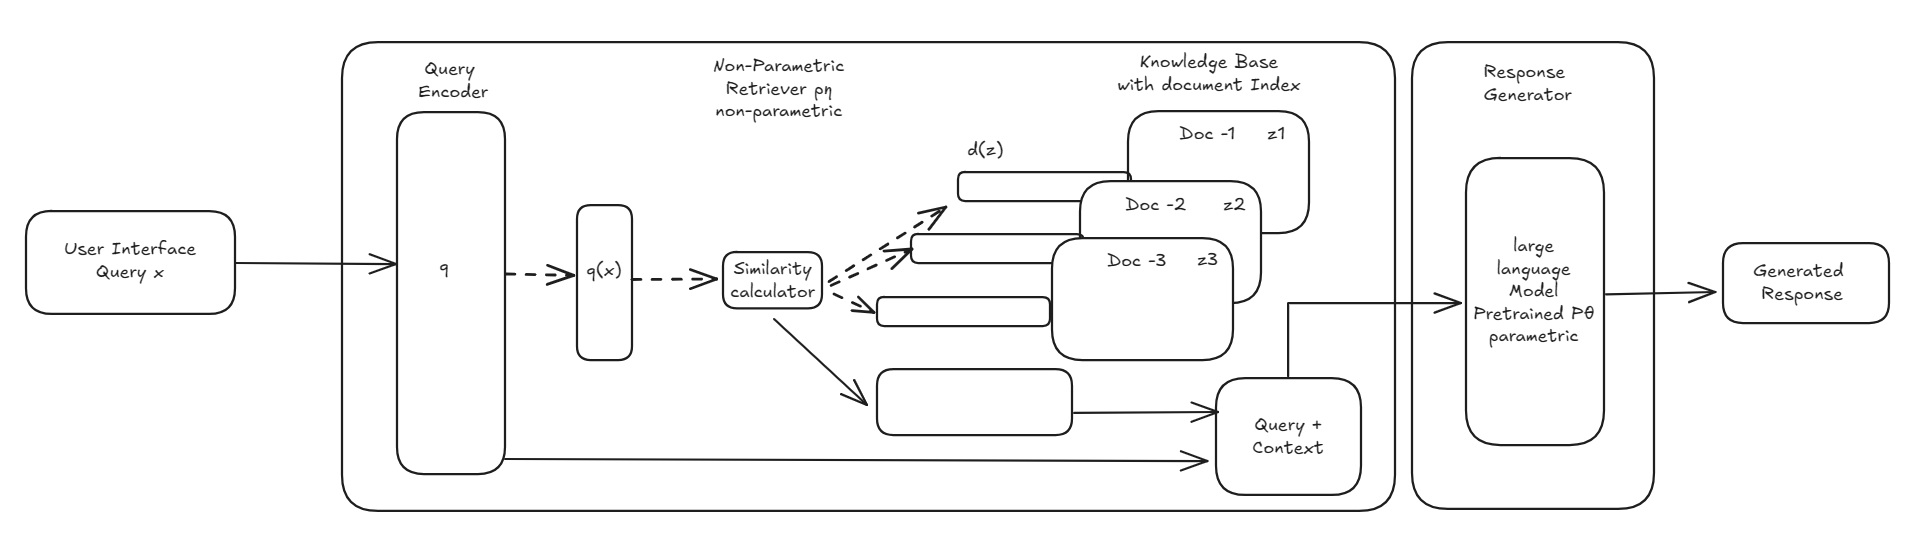
\includegraphics[width=\linewidth]{RAG_Architecture.jpg}
    \captionsetup{justification=centering}
    \caption{Proposed Chatbot Architecture}
    \label{fig:example}
\end{figure}

As depicted in Figure 1, the system first takes a user query and uses the retrieval module to identify the top five most relevant documents from the knowledge base. These retrieved documents, along with the original user query, are then fed into the large language model to generate the response.

\subsection{Retrieval Module}
The retrieval component of our chatbot operates as follows:

\begin{itemize}
    \item \textbf{Knowledge Base:} Our knowledge base is the MS MARCO\cite{MS_MARCO} dataset, an open-source, human-generated machine reading comprehension dataset curated for question answering.
    \item \textbf{Embedding Generation:} To represent both user queries and documents within the MS MARCO dataset as dense vectors, we utilize the \textbf{Sentence Transformer all-MiniLM-L6-v2}\cite{MiniLm} model. This model is known for generating effective sentence embeddings.
    \item \textbf{Indexing and Similarity Search:} For efficient storage and retrieval of these vector embeddings, we employ the \textbf{FAISS}. Specifically, we use the \texttt{IndexFlatL2}\cite{faisslibrary} index, which performs a flat (brute-force) $k$-nearest neighbors search based on the Euclidean distance ($L_2$ norm) between the query vector and the document vectors.
    \item \textbf{Retrieval Process:} When a user inputs a query ($X_q$), it is first encoded into an embedding $Q(X_q)$ using the Sentence Transformer model. We then calculate the Euclidean distance between this query embedding and all document embeddings within our FAISS index. The top five documents with the smallest Euclidean distances (i.e., the most similar) are retrieved as context.
\end{itemize}
\subsection{Large Language Model for Generation}

The generative component of our chatbot is powered by the \texttt{microsoft/phi-3-mini-instruct}\cite{Microsoft_Phi} model. This instruction-tuned LLM is designed for high-quality reasoning and was trained on a publicly available dataset. The retrieved top five documents, along with the original user query, are provided as context to this parameterized LLM ($P_{\theta}$) to generate a relevant and informative response. The LLM processes both the non-parametric memory (retrieved documents) and its internal parametric knowledge to produce the final output.

\subsection{Implementation Details}
While we initially planned to deploy this chatbot as a Flask application for broader accessibility, time constraints led us to implement it as a Jupyter Notebook for the present study. We intend to transition to a Flask-based deployment in future work.

In summary, our system takes a user query, encodes it into a vector embedding, retrieves the top five most similar documents from our pre-processed MS MARCO \cite{MS_MARCO} knowledge base using Euclidean distance via FAISS\cite{faisslibrary}, and then provides the query and retrieved documents as context to the \texttt{microsoft/phi-3-mini-instruct}\cite{Microsoft_Phi} model to generate a response within a Jupyter Notebook environment for this study.

\subsection{Experimental Setup}

\subsubsection{Retrieval Parameter Exploration}

While our current implementation uses the Euclidean distance metric, future experiments could explore the impact of more advanced, attention-based, and neural network-based similarity metrics on retrieval performance.

\subsubsection{Document Chunking Strategy Evaluation}

We conducted experiments by randomly sampling 50 questions from the dataset to evaluate the impact of different document chunking strategies on the quality of the generated responses. We compared two main approaches: fixed-size chunking and recursive character chunking, further exploring the effect of overlap within recursive chunking.

\begin{itemize}
    \item \textbf{Fixed-Size Chunking:}
    We experimented with a fixed chunk length of 200 tokens as one of our baseline strategies.

    \item \textbf{Recursive Character Chunking with Overlap:}
    We investigated the impact of introducing overlap between consecutive chunks for the recursive character chunking strategy. Overlap refers to the number of common words shared between two adjacent chunks. We experimented with three different overlap percentages: 0\% overlap, 20\% overlap, and 50\% overlap. The rationale behind exploring overlap is to provide the language model with more contextual continuity across retrieved segments, potentially leading to improved coherence and more informative generated answers.
\end{itemize}.

These experiments aimed to determine the optimal chunking strategy and overlap configuration for providing sufficient context to the language model and improving the coherence and informativeness of the generated answers.

\subsection{Evaluation Metric}

We evaluated the performance of our question answering system using the ROUGE-L metric. This metric measures the length of the longest common subsequence (LCS) between the generated answer and the human-generated reference answer in the MS MARCO\cite{MS_MARCO} dataset, providing an indication of the factual overlap and alignment. Specifically, the ROUGE-L Recall is calculated as:

$$
\text{ROUGE-L Recall} = \frac{\text{Length of LCS}}{\text{Total number of words in the reference text}}
$$

This recall value indicates the proportion of words in the reference answer that are also present in the generated answer, considering their sequential order.
\section{Results}

\subsection{Quantitative Evaluation of Chunking Strategies}

To quantitatively evaluate the impact of different document chunking strategies on the performance of our RAG-based question answering system, we calculated the ROUGE-L scores for 50 randomly sampled questions from the MS MARCO dataset. The descriptive statistics for each chunking strategy are summarized in Table~\ref{fig:rouge_results} and visualized in Figure~\ref{fig:boxplot}.


\begin{figure}[H]
    \centering

    \begin{minipage}[t]{0.48\textwidth}
        \centering
        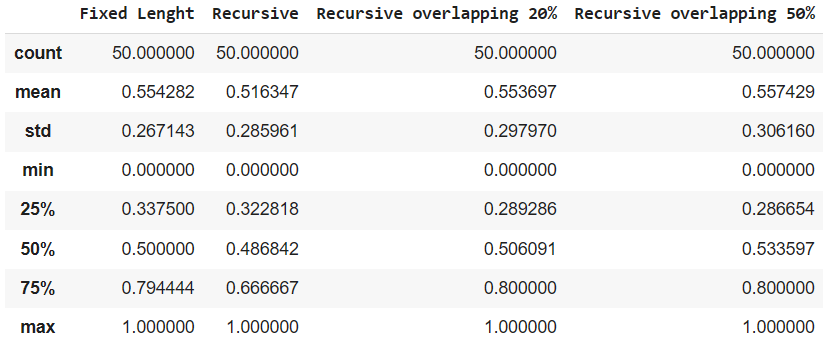
\includegraphics[height=3cm]{Results_discription.png}
        \caption{Descriptive Statistics of ROUGE-L Scores}
        \label{fig:rouge_results}
    \end{minipage}%
    \hfill
    \begin{minipage}[t]{0.48\textwidth}
        \centering
        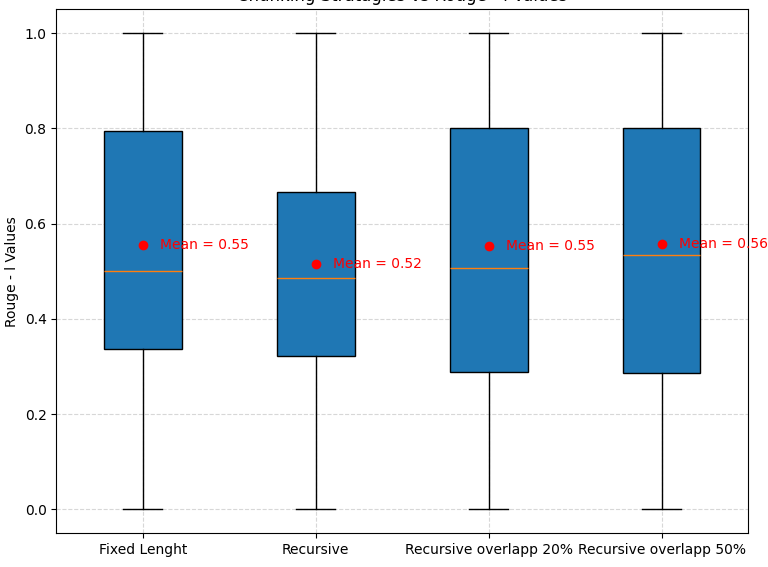
\includegraphics[height=3cm]{Results_Box.png}
        \caption{Box Plot Comparison of ROUGE-L Scores}
        \label{fig:boxplot}
    \end{minipage}

\end{figure}



The box plot (Figure~\ref{fig:boxplot}) visually compares the distribution of ROUGE-L scores across the four chunking strategies. The numerical statistics in Table~\ref{fig:rouge_results} provide a more detailed breakdown of these distributions, including the mean, standard deviation, quartiles, and range.

\subsection{Visual Comparison of Performance Distribution}

As illustrated in Figure~\ref{fig:boxplot}, the spread of ROUGE-L scores varies across the different chunking methods. The Recursive strategy exhibits a slightly lower median and a narrower upper quartile compared to the other methods. Conversely, the Recursive strategies with 20\% and 50\% overlap show comparable or slightly better median and upper quartile values than the Fixed Length approach. The lower whiskers suggest that the overlapping recursive strategies might have fewer instances of extremely low performance compared to the standard Recursive method.

\section{Conclusion and Future Directions}

Based on our observations, the choice of document chunking strategy significantly impacts the performance of the RAG-based question answering system, as measured by the ROUGE-L score. While the average performance is relatively close, the introduction of overlap within the recursive chunking method demonstrates a promising avenue for improvement. Specifically, the recursive strategy with a 50\% overlap yielded the highest mean and median ROUGE-L scores across our evaluation set. This suggests that providing more continuous contextual information to the language model can lead to better alignment with the reference answers.

Furthermore, it is important to highlight that our RAG-based chatbot, even with minimal training resources, demonstrates the capability to produce quality-based output, achieving encouraging ROUGE-L scores. This underscores the potential of the architecture to leverage readily available pre-trained models and external knowledge effectively, reducing the need for extensive task-specific training while still delivering high-quality results.

However, the substantial variability in scores across all strategies indicates that the optimal chunking approach might be context-dependent. For future work, we recommend conducting a more in-depth analysis of the questions and documents where different chunking strategies perform particularly well or poorly. Furthermore, exploring a wider range of overlap percentages and fixed chunk sizes, as well as investigating more sophisticated, semantic-aware chunking techniques, could potentially lead to further performance enhancements and a more robust and consistent question answering system. Additionally, conducting statistical significance tests to validate the observed trends and performing qualitative evaluations of the generated responses would provide a more comprehensive understanding of the impact of different chunking strategies. Finally, exploring the trade-offs between computational resources, training requirements, and the quality of the generated output remains a crucial direction for future research in this area.

\bibliographystyle{abbrvnat}
\bibliography{RAG}


\end{document}
